\begin{figure}[H]
    \centering
    \definecolor{coreorange}{RGB}{225,120,55}
    \definecolor{mantleblue}{RGB}{95,155,205}
    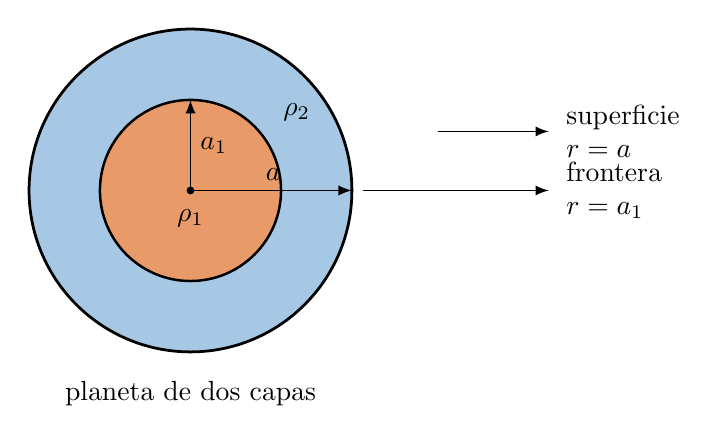
\begin{tikzpicture}[x=1cm,y=1cm,line cap=round,line join=round]
        \coordinate (O) at (4.0,2.35);
        \fill[mantleblue!55] (O) circle (2.05);
        \fill[coreorange!75] (O) circle (1.15);
        \draw[line width=1.0pt] (O) circle (2.05);
        \draw[line width=0.9pt] (O) circle (1.15);
        \fill (O) circle (0.05);

        \draw[-latex,line width=0.7pt] (O) -- ++(2.05,0);
        \node[above] at (5.05,2.35) {$a$};
        \draw[-latex,line width=0.7pt] (O) -- ++(0,1.15);
        \node[right] at (4.00,2.92) {$a_1$};

        \node at (4.0,2.0) {$\rho_1$};
        \node at (5.35,3.35) {$\rho_2$};
        \node[below] at (4.0,0.05) {planeta de dos capas};

        \draw[-latex,line width=0.65pt] (7.15,3.10) -- (8.55,3.10);
        \node[right,align=left] at (8.65,3.10)
            {superficie\\$r=a$};
        \draw[-latex,line width=0.65pt] (6.20,2.35) -- (8.55,2.35);
        \node[right,align=left] at (8.65,2.35)
            {frontera\\$r=a_1$};
    \end{tikzpicture}
    \caption{Modelo esférico de dos capas con densidades constantes $\rho_1$ y $\rho_2$.}
\end{figure}